% arXiv decides between latex+dvips and pdflatex by scanning the first few
% lines of the source.  Every figure here is a committed PDF, so the choice is
% pinned to pdflatex rather than left to inference.
\pdfoutput=1

\documentclass[aps,pra,reprint,superscriptaddress,nofootinbib,floatfix,
  showkeys]{revtex4-2}

\usepackage{amsmath,amssymb,bm}
\usepackage{graphicx}
\usepackage{microtype}
\usepackage{xcolor}
\usepackage[colorlinks=true,linkcolor=blue,citecolor=blue,urlcolor=blue]{hyperref}
\hypersetup{
  pdftitle={How compact is a compact subspace? Columns, Hamiltonian actions and
    determinant support in a preregistered test of residual packets},
  pdfauthor={Ginanjar Utama and Hermawan Kresno Dipojono},
  pdfsubject={Adaptive subspace eigensolvers, selected configuration
    interaction, Davidson method, preregistered negative result}
}

\newcommand{\pkg}{\texttt{clifford\_qc}}
\newcommand{\ket}[1]{\lvert #1\rangle}
\newcommand{\bra}[1]{\langle #1\rvert}
% Narrower column gaps for the wide tables; a length typed into the body would
% read as a hand-typed number to the manuscript gate.
\newcommand{\tightcolumns}{\setlength{\tabcolsep}{3.2pt}}

\raggedbottom
\makeatletter
\setlength{\@fptop}{0pt}
\setlength{\@fpsep}{14pt plus 0fil}
\setlength{\@fpbot}{0pt plus 1fil}
\setlength{\@dblfptop}{0pt}
\setlength{\@dblfpsep}{14pt plus 0fil}
\setlength{\@dblfpbot}{0pt plus 1fil}
\makeatother
\renewcommand{\dbltopfraction}{0.75}
\renewcommand{\topfraction}{0.8}
\renewcommand{\textfraction}{0.1}
\renewcommand{\dblfloatpagefraction}{0.9}
\renewcommand{\floatpagefraction}{0.85}

% Every quantity in the body text is generated from a committed record; see
% the reproducibility section.
% source-git-blob-sha: 70da4d0015b3a81b50b63ea41cb8ce9c4799f6a8
% source-git-blob-sha: 15de9b3aa7a81b11fd2875abc0b6d17d1d9a0c31
% source-git-blob-sha: 452778c6e5459ea49ff4b7c712aeb6f848fedbaa
% source-git-blob-sha: 6e2f6da87ed8f0a0ebfd9af688a3a2574020b6e0
% source-git-blob-sha: 178bd5fd9c391703a17241da8c3f9196a42cc3a0
% source-git-blob-sha: abe9d543d8558786e55a2ca957642b9453799f2a
% source-git-blob-sha: 3a9a7d874cb53619293f51cf0a6a51809234587d
% source-git-blob-sha: 55418ea5bd2206a7e012b32493c804c66f1633bb
% generator-git-blob-sha: daabb897d72e67a564233dae3804d4d1e6607db2
\newcommand{\pkAuditInterval}{five}
\newcommand{\pkBerylliumColumnRatioTight}{\ensuremath{0.91}}
\newcommand{\pkBerylliumColumnsTenth}{\ensuremath{4}}
\newcommand{\pkBerylliumDavidsonColumnsTight}{\ensuremath{6}}
\newcommand{\pkBerylliumDavidsonSupportTight}{\ensuremath{171}}
\newcommand{\pkBerylliumPacketsActionsTenth}{\ensuremath{32}}
\newcommand{\pkBerylliumPacketsColumnsTight}{\ensuremath{20}}
\newcommand{\pkBerylliumPacketsSupportTight}{\ensuremath{35}}
\newcommand{\pkBerylliumSciActionsTenth}{\ensuremath{490}}
\newcommand{\pkBerylliumSciColumnsTight}{\ensuremath{22}}
\newcommand{\pkCacheCells}{\ensuremath{84}}
\newcommand{\pkCacheMinimumReduction}{\ensuremath{20\%}}
\newcommand{\pkCachePayloads}{eight}
\newcommand{\pkCacheReduction}{\ensuremath{44.41\%}}
\newcommand{\pkCacheRssGrowth}{\ensuremath{4.37\%}}
\newcommand{\pkCells}{\ensuremath{52}}
\newcommand{\pkChainDavidsonColumnsTight}{\ensuremath{23}}
\newcommand{\pkChainDavidsonSupportTight}{\ensuremath{4{,}436}}
\newcommand{\pkChainEarlyFinalError}{\ensuremath{0.00565}}
\newcommand{\pkChainMinActionRatio}{\ensuremath{5.4}}
\newcommand{\pkChainName}{$1{\times}8$ Hubbard chain}
\newcommand{\pkChainPacketThresholds}{\ensuremath{1}, \ensuremath{0.1} and \ensuremath{0.01}}
\newcommand{\pkChainPacketsColumns}{\ensuremath{89}, \ensuremath{251} and \ensuremath{484}}
\newcommand{\pkChainPacketsFinalError}{\ensuremath{0.00762}}
\newcommand{\pkChainPacketsSupportOne}{\ensuremath{842}}
\newcommand{\pkChainPacketsSupportTenth}{\ensuremath{2{,}244}}
\newcommand{\pkChainSciColumns}{\ensuremath{166} and \ensuremath{404}}
\newcommand{\pkChainSciSupportOne}{\ensuremath{942}}
\newcommand{\pkChainSciSupportTenth}{\ensuremath{1{,}474}}
\newcommand{\pkChainStartWeight}{\ensuremath{<10^{-12}}}
\newcommand{\pkCompactRatio}{\ensuremath{0.8}}
\newcommand{\pkCompleteSpanTolerance}{\ensuremath{10^{-8}}}
\newcommand{\pkCoordinateEarlyReduction}{\ensuremath{36.8\%}}
\newcommand{\pkCoordinateExhaustiveReduction}{\ensuremath{50.2\%}}
\newcommand{\pkCoordinateSwapSteps}{\ensuremath{28}, \ensuremath{31}, \ensuremath{32} and \ensuremath{36}}
\newcommand{\pkEarlyColumnRatio}{\ensuremath{1.1}}
\newcommand{\pkEarlyFrontierBand}{\ensuremath{10\%}}
\newcommand{\pkFrontierList}{\ensuremath{64}, \ensuremath{128} and \ensuremath{256}}
\newcommand{\pkFrontierMinimum}{\ensuremath{128}}
\newcommand{\pkFullReplayDimension}{\ensuremath{1{,}225}}
\newcommand{\pkInputCount}{five}
\newcommand{\pkLadderDavidsonColumnsTight}{\ensuremath{15}}
\newcommand{\pkLadderEarlyAudits}{five}
\newcommand{\pkLadderEarlyErrorChange}{\ensuremath{12.85\%}}
\newcommand{\pkLadderEarlyMissed}{two}
\newcommand{\pkLadderInteraction}{\ensuremath{8}}
\newcommand{\pkLadderName}{$2{\times}3$ Hubbard lattice}
\newcommand{\pkLadderPacketsColumnsTight}{\ensuremath{102}}
\newcommand{\pkLadderSciColumnsTight}{\ensuremath{135}}
\newcommand{\pkLargeBudget}{\ensuremath{64}}
\newcommand{\pkLargePacketsError}{\ensuremath{1.94}}
\newcommand{\pkLargeSciError}{\ensuremath{2.08}}
\newcommand{\pkLargeSciSeconds}{\ensuremath{6.86}}
\newcommand{\pkMaxRepeats}{three}
\newcommand{\pkMinRepeats}{two}
\newcommand{\pkPayloads}{\ensuremath{20}}
\newcommand{\pkPrimaryActionRatio}{\ensuremath{122}}
\newcommand{\pkPrimaryColumnRatioOne}{\ensuremath{0.83}}
\newcommand{\pkPrimaryDavidsonColumnsOne}{\ensuremath{21}}
\newcommand{\pkPrimaryDavidsonError}{\ensuremath{0.9949}}
\newcommand{\pkPrimaryDavidsonOverlap}{\ensuremath{1.5\times10^{-12}}}
\newcommand{\pkPrimaryDavidsonResidual}{\ensuremath{9.2\times10^{-9}}}
\newcommand{\pkPrimaryDavidsonStopColumns}{\ensuremath{48}}
\newcommand{\pkPrimaryDavidsonSupportOne}{\ensuremath{4{,}720}}
\newcommand{\pkPrimaryDeterminants}{\ensuremath{4{,}900}}
\newcommand{\pkPrimaryEarlyActionFactor}{\ensuremath{2.3}}
\newcommand{\pkPrimaryEarlyActions}{\ensuremath{93{,}131}}
\newcommand{\pkPrimaryGap}{\ensuremath{0.917}}
\newcommand{\pkPrimaryInteraction}{\ensuremath{4}}
\newcommand{\pkPrimaryMatchedColumns}{\ensuremath{48}}
\newcommand{\pkPrimaryName}{$2{\times}4$ Hubbard lattice}
\newcommand{\pkPrimaryPacketsActions}{\ensuremath{215{,}421}}
\newcommand{\pkPrimaryPacketsColumnsOne}{\ensuremath{145}}
\newcommand{\pkPrimaryPacketsColumnsTenth}{\ensuremath{473}}
\newcommand{\pkPrimaryPacketsFinalError}{\ensuremath{0.0763}}
\newcommand{\pkPrimaryPacketsSupportMatched}{\ensuremath{676}}
\newcommand{\pkPrimaryPacketsSupportOne}{\ensuremath{1{,}696}}
\newcommand{\pkPrimarySciActions}{\ensuremath{1{,}764}}
\newcommand{\pkPrimarySciColumnsOne}{\ensuremath{174}}
\newcommand{\pkPrimarySciFinalError}{\ensuremath{0.248}}
\newcommand{\pkPrimarySciSupportMatched}{\ensuremath{396}}
\newcommand{\pkPrimarySciSupportOne}{\ensuremath{1{,}010}}
\newcommand{\pkPrimarySpinBlock}{\ensuremath{70}}
\newcommand{\pkPrimaryStartWeight}{\ensuremath{1.7\times10^{-6}}}
\newcommand{\pkResidualTolerance}{\ensuremath{10^{-9}}}
\newcommand{\pkReuseActionsAfter}{\ensuremath{1{,}301}}
\newcommand{\pkReuseActionsBefore}{\ensuremath{10{,}841}}
\newcommand{\pkReuseRssAfter}{\ensuremath{897}}
\newcommand{\pkReuseRssBefore}{\ensuremath{684}}
\newcommand{\pkReuseSecondsAfter}{\ensuremath{43.4}}
\newcommand{\pkReuseSecondsBefore}{\ensuremath{27.9}}
\newcommand{\pkShift}{\ensuremath{0.1}}
\newcommand{\pkShortlistErrorChange}{\ensuremath{0.51\%}}
\newcommand{\pkShortlistFraction}{\ensuremath{80\%}}
\newcommand{\pkSparseDeclaredReduction}{\ensuremath{20\%}}
\newcommand{\pkSparseReduction}{\ensuremath{5.6\%}}
\newcommand{\pkSparseRssAfter}{\ensuremath{181}}
\newcommand{\pkSparseRssBefore}{\ensuremath{686}}
\newcommand{\pkStartColumns}{three}
\newcommand{\pkStartSpace}{CAS(2e,2o)}
\newcommand{\pkSupportTolerance}{\ensuremath{10^{-12}}}
\newcommand{\pkThresholdList}{\ensuremath{1}, \ensuremath{0.1}, \ensuremath{0.01} and \ensuremath{0.0016}}
\newcommand{\pkThresholdOne}{\ensuremath{1}}
\newcommand{\pkThresholdTenth}{\ensuremath{0.1}}
\newcommand{\pkThresholdTight}{\ensuremath{0.0016}}
\newcommand{\pkTieTolerance}{\ensuremath{10^{-12}}}
\newcommand{\pkTightTarget}{\ensuremath{1.6}\,mHa}
\newcommand{\pkWaterName}{H$_2$O CAS(8e,6o)}
\newcommand{\pkWaterPacketActions}{\ensuremath{213}}
\newcommand{\pkWaterPacketColumns}{\ensuremath{12}}
\newcommand{\pkWaterPacketScores}{\ensuremath{210}}
\newcommand{\pkWaterReuseActions}{\ensuremath{57}}
\newcommand{\pkWaterSciActions}{\ensuremath{105}}
\newcommand{\pkWaterSciColumns}{\ensuremath{14}}
\newcommand{\pkWaterShortlistScores}{\ensuremath{63}}
\newcommand{\pkWorkRatio}{\ensuremath{1.25}}
\newcommand{\pkWorkerTimeout}{\ensuremath{3{,}600}}


\begin{document}

\title{How Compact Is a Compact Subspace? Columns, Hamiltonian Actions and
Determinant Support in a Preregistered Test of Residual Packets}

\author{Ginanjar Utama}
\email{ginanjar.utama@gmail.com}
\affiliation{Department of Engineering Physics, Institut Teknologi Bandung,
Bandung, Indonesia}

\author{Hermawan Kresno Dipojono}
\email{dipojono@itb.ac.id}
\affiliation{Department of Engineering Physics, Institut Teknologi Bandung,
Bandung, Indonesia}

\date{October 30, 2026}

\begin{abstract}
Adaptive subspace eigensolvers are usually compared by how many basis vectors
they need. What a basis vector costs also depends on how much work selected it
and on how many determinants it occupies. We compare three ways of growing a
spin-adapted subspace one column at a time---greedy selected configuration
interaction (CI), residual packets that confine a preconditioned residual to
one group of configuration-state functions sharing an occupation pattern, and
an unrestricted Davidson correction---under three yardsticks: retained columns,
Hamiltonian actions, and determinant support. The comparison was declared
before implementation, executed in \pkCells{} fresh processes on
\pkInputCount{} exact classical sectors that include held-out lattice and
molecular inputs, and replayed independently. Under the declared column rule,
packets add no compactness over selected CI: the primary \pkPrimaryName{} and
the held-out stretched BeH$_2$ read mixed, and only the held-out
\pkChainName{} favours packets, at \pkChainMinActionRatio{} or more times
selected CI's Hamiltonian actions. Davidson needs far fewer columns wherever it
reaches the ground state, but its columns spread over almost the whole sector,
and on the primary lattice it stopped on an excited singlet. Davidson leads in
columns and actions and never in support; between the two bounded-support
rules the support lead changes hands. Exact engineering that roughly halved
the packet arm's run time left its column verdict unchanged. A compactness
claim therefore needs a cost model declared in advance; packets could pay off
only under one that prices bounded column support, which these exact classical
simulations do not test.
\end{abstract}

\keywords{subspace diagonalization; selected configuration interaction;
Davidson method; spin adaptation; Hubbard model; quantum subspace methods;
preregistration; negative results}

\maketitle

\section{Introduction}
\label{sec:introduction}

Subspace eigensolvers approximate a low-lying eigenpair of a large Hamiltonian
by diagonalizing it in a small basis grown one piece at a time. Selected
configuration interaction (CI) adds determinants or configuration-state
functions (CSFs) chosen by an importance criterion~\cite{huron1973cipsi,
holmes2016hci}; Davidson's method adds a preconditioned
residual~\cite{davidson1975iterative}; and quantum subspace methods build the
basis from states prepared or sampled on a quantum
processor~\cite{mcclean2017qse,stair2020krylov,kanno2026qsci,
robledomoreno2025sqd}. The usual figure of merit is the dimension the basis
needs to reach a target accuracy. Dimension does matter: it fixes the size of
the projected eigenproblem and, when matrix elements are estimated rather than
computed, the number of quantities to estimate~\cite{epperly2022theory,
lee2024sampling}.

Dimension is not the whole cost, however. Two further quantities decide what
a basis vector costs. One is the work spent choosing it: a greedy rule that
scores many candidates applies the Hamiltonian to each of them, and that work
is spent whether or not a candidate is kept. The other is what the vector is:
a single determinant, a CSF on a handful of determinants, or a dense
combination spread over the sector. Its support decides how it is stored, how
its matrix elements are formed, and whether a method can leave the regime of
explicit sector vectors at all. In sampled-determinant methods the two
coincide, because every basis vector is a determinant and dimension and
support are the same number~\cite{kanno2026qsci,robledomoreno2025sqd}. They
separate as soon as basis vectors are combinations.

This paper is about that separation, studied through one method that sits
between the extremes. Residual packets confine a Davidson-type preconditioned
residual to one group of spin-adapted CSFs that share their occupation outside
a small active space, and add the best such group direction as one new column.
Packets arose in the development of the open-source \pkg{}
toolkit~\cite{utama2026architecture}, in exact small-sector pilots. On an
\pkWaterName{} active space they reached a \pkTightTarget{} target
in \pkWaterPacketColumns{} columns against selected CI's
\pkWaterSciColumns{}, but after \pkWaterPacketActions{} Hamiltonian actions
against \pkWaterSciActions{}. On a \pkPrimaryDeterminants{}-determinant Hubbard
sector with a budget of \pkLargeBudget{} columns, both methods stayed far from
the reference: packets ended \pkLargePacketsError{}\,$t$ above it and selected
CI \pkLargeSciError{}\,$t$. Whether the packets' column advantage would survive
larger budgets, and at what price, was open.

We settled the question with a comparison declared before any of its code
existed~\cite{nosek2018preregistration}. Its question was narrow on purpose:
do packets need fewer columns than greedy selected CI? The answer is no. What
makes the outcome worth reporting is how it reads under the other two
yardsticks. The same trajectories rank the arms differently by columns, by
Hamiltonian actions, and by determinant support. The unrestricted Davidson
correction, included as a reference, wins the first two by an order of
magnitude and loses the third, and on the primary input it converged to the
wrong root.

The contributions are:
(i) three yardsticks for adaptive subspace growth, and the placement of three
growth rules along a spectrum of column support (Sec.~\ref{sec:yardsticks});
(ii) a preregistered column-budget comparison on exact sectors with held-out
lattice and molecular inputs and independent replay
(Sec.~\ref{sec:declared});
(iii) the result that packets add no column compactness under the declared
rule, together with the rank changes across yardsticks that the rule alone
would hide (Sec.~\ref{sec:results});
(iv) a ledger of exact and heuristic engineering on the packet arm, which
reduced its time, memory or work without moving its column verdict
(Sec.~\ref{sec:ledger}); and
(v) the cost model under which packets could still matter, and why these
simulations cannot test it (Sec.~\ref{sec:discussion}).

Every calculation is an exact classical computation with explicit sector
vectors on a small sector. Nothing here measures a matrix element on a
device, compares against an optimized selected CI such as heat-bath
CI~\cite{holmes2016hci}, or claims asymptotic scaling.

\section{Three yardsticks}
\label{sec:yardsticks}

\subsection{Setting}

Let $H$ be a Hamiltonian restricted to the sector of fixed particle number and
zero spin projection, with $D$ determinants. A singlet frame
$F\in\mathbb{C}^{D\times F_s}$ holds orthonormal CSFs of total spin zero. It is
built block by block: determinants that share a spatial occupation pattern
span an $S^2$-invariant block, and the canonically oriented singlet
eigenvectors of each block are the frame columns~\cite{pauncz1979spin}. Every
frame column is therefore supported on one block, of at most
\pkPrimarySpinBlock{} determinants on the largest inputs here. After the
determinants are ordered by spatial pattern, $F$ is block diagonal.

Each growth rule below keeps an orthonormal basis $V_k$ of $k$ columns in the
range of $F$, the Hamiltonian actions $HV_k$, and the lowest Ritz pair
$(E_k,\ket{\psi_k})$ of $V_k^\dagger H V_k$ with true residual
$\ket{r_k}=H\ket{\psi_k}-E_k\ket{\psi_k}$. A step appends one unit vector
orthogonal to $V_k$.

\subsection{What is counted}

We record three quantities at every prefix of every trajectory.
\emph{Columns} $K=k$ is the subspace dimension.
\emph{Actions} $W$ is the cumulative number of products $Hv$ with a sector
vector $v$, counting every candidate whose action was computed, selected or
not. Inner products and the $k$-dimensional Ritz solves are not counted; on
these sectors they are cheap, though not free.
\emph{Support} $S$ is the number of determinants on which some column of $V_k$
has an amplitude larger than \pkSupportTolerance{} in magnitude---the size of
the union of the column supports.

Classically, $K$ sets the size of the projected problem and the number of
stored vectors, $W$ dominates the run time whenever a Hamiltonian action is
the expensive operation, and $S$ bounds the storage of a sparse representation
of the span. In a measured setting the readings change: $K^2$ matrix elements
must be estimated, and the support of a column, not its index, determines what
must be prepared or sampled to estimate them. We do not test that reading. It
is why support is reported at all.

\subsection{Three growth rules}

All three rules start from the same span and differ in one respect: how much
of the residual a single new column may carry (Fig.~\ref{fig:spectrum}).

\begin{figure}[t]
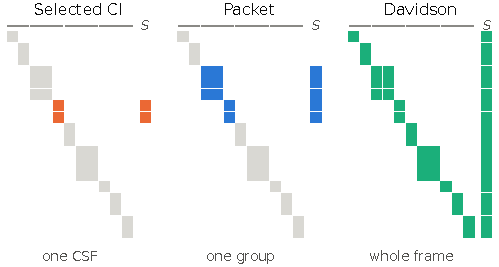
\includegraphics[width=\columnwidth]{paper_assets/support_spectrum.pdf}
\caption{What one new column may contain. Squares are nonzero entries of an
illustrative singlet frame (determinants down, CSFs across), block diagonal by
spatial occupation; bars above group the CSFs by occupation outside the
active space. Selected CI adds one CSF, a packet combines one group, and
Davidson combines the whole frame. The column marked $S$ shows the
determinants the new column can occupy. Schematic; it plots no record.}
\label{fig:spectrum}
\end{figure}

\emph{Selected CI} adds one frame column per step. Every unselected column
$\ket{f_j}$ is a candidate; because the frame is orthonormal and the span
consists of frame columns, $\ket{f_j}$ is already orthogonal to $V_k$. A
candidate $\ket{d}$ is scored by the exact lowering it would produce together
with $\ket{\psi_k}$,
\begin{equation}
\Delta(d)=\tfrac{1}{2}\Bigl[\sqrt{g^2+4\lvert c\rvert^2}-g\Bigr],
\label{eq:lowering}
\end{equation}
with $g=\bra{d}H\ket{d}-E_k$ and $c=\bra{\psi_k}H\ket{d}$. This is the drop of the lowest eigenvalue of the two-by-two projection of
$H$ onto $\{\ket{\psi_k},\ket{d}\}$ below $E_k$. The candidate with the
largest $\Delta$ is added, ties within \pkTieTolerance{} broken by column
index. A candidate's action is computed when it is first scored and then
kept, so after the first step $W$ equals the frame dimension $F_s$: this
selected CI pays for the complete frame action table up front. It is greedy,
spin-adapted selected CI, not an optimized variant with perturbative
selection~\cite{huron1973cipsi,holmes2016hci}.

\emph{Residual packets} partition the frame columns outside the starting span
into groups $G_g$ whose CSFs share one occupation pattern outside the active
space. A step forms the diagonally preconditioned residual
\begin{equation}
\ket{t_k}=\frac{\ket{r_k}}{\max\bigl(\operatorname{diag}H-E_k+\sigma,\;\sigma\bigr)},
\qquad \sigma=\pkShift{},
\label{eq:preconditioned}
\end{equation}
with the division taken entrywise, and for every group the candidate
\begin{equation}
\ket{d_g}\propto\bigl(I-V_kV_k^\dagger\bigr)F_gF_g^\dagger\ket{t_k},
\label{eq:packet}
\end{equation}
orthogonalized twice and rejected below a relative norm cutoff. Each
candidate costs one action, and the one with the largest $\Delta(d_g)$ is
added. A packet column is supported on the union of its group's blocks. An
early policy screens groups by their residual mass, keeps the smallest set
that holds \pkShortlistFraction{} of it, audits every group once every
\pkAuditInterval{} steps, and falls back to all groups when the shortlist
gains nothing. It is a heuristic.

\emph{Davidson} merges every group into one direction,
\begin{equation}
\ket{d}\propto\bigl(I-V_kV_k^\dagger\bigr)FF^\dagger\ket{t_k},
\label{eq:davidson}
\end{equation}
with the packets' preconditioner and cutoffs. It spends one action per step,
and its columns may cover the whole sector.

Read together, Eqs.~\eqref{eq:packet} and~\eqref{eq:davidson} place the rules
on one axis. A packet is the Davidson direction confined to one group. A
selected-CI candidate is the Davidson direction confined to one CSF, since
$(I-V_kV_k^\dagger)\ket{f_j}\bra{f_j}t_k\rangle$ is proportional to
$\ket{f_j}$; the only difference is that selected CI scores every CSF,
including those the residual does not touch. Confinement buys bounded column
support and costs either columns or candidate actions; Davidson is the
reference that measures how much.

\section{The declared comparison}
\label{sec:declared}

\subsection{Declaration and inputs}

The design was committed before any of its implementation: arms, inputs,
budgets, thresholds, stopping rules, readouts and the decision rule were fixed
in a machine-readable configuration~\cite{nosek2018preregistration}. One
revision preceded execution. A toy Hubbard test, run before any campaign input,
showed lowest-root Davidson converging to an excited singlet when its start
had no ground-state overlap, so the revision added a diagnostic: every arm's
final overlap with the reference ground space, computed after timing. The
arms and readouts did not change.

Table~\ref{tab:inputs} lists the inputs. The primary input is the open
\pkPrimaryName{} at half filling with $U/t=\pkPrimaryInteraction$; the
held-out lattice is the open \pkChainName{} with the same parameters and the
same sector and frame dimensions, which no packet arm had run before. The
held-out molecule is the full STO-3G sector of BeH$_2$ symmetrically stretched
to twice its equilibrium bond length; a different, sampled packet family had run only on an active
space of that geometry. The smaller inputs serve as complete-span controls:
the open \pkLadderName{} with $U/t=\pkLadderInteraction$ and the
\pkWaterName{} development input. Hubbard models follow the standard
convention~\cite{hubbard1963electron}; molecular Hamiltonians are read from
integral files~\cite{knowles1989fcidump}.

\begin{table*}[t]
\caption{Inputs. Determinants and singlet columns are the sector and frame
dimensions; groups count the packet groups outside the starting span. The
budget is the column ceiling. The last column is the largest ground-space
weight in the shared starting span, computed independently after
observation; a value below the frame's numerical floor is rounding.}
\label{tab:inputs}
\begin{ruledtabular}
\begin{tabular}{llrrrrlr}
Input & Role & Determinants & Singlet columns & Groups & Budget & Unit & Start weight \\
\hline
% source-git-blob-sha: 70da4d0015b3a81b50b63ea41cb8ce9c4799f6a8
% source-git-blob-sha: 15de9b3aa7a81b11fd2875abc0b6d17d1d9a0c31
% generator-git-blob-sha: daabb897d72e67a564233dae3804d4d1e6607db2
$2{\times}4$ Hubbard & primary & \ensuremath{4{,}900} & \ensuremath{1{,}764} & \ensuremath{572} & \ensuremath{512} & $t$ & \ensuremath{1.7\times10^{-6}} \\
$1{\times}8$ Hubbard chain & held-out lattice & \ensuremath{4{,}900} & \ensuremath{1{,}764} & \ensuremath{572} & \ensuremath{512} & $t$ & \ensuremath{<10^{-12}} \\
BeH$_2$, stretched & held-out molecule & \ensuremath{1{,}225} & \ensuremath{490} & \ensuremath{185} & \ensuremath{490} & Ha & \ensuremath{0.76} \\
$2{\times}3$ Hubbard & complete-span control & \ensuremath{400} & \ensuremath{175} & \ensuremath{70} & \ensuremath{175} & $t$ & \ensuremath{7.1\times10^{-6}} \\
H$_2$O CAS(8e,6o) & development control & \ensuremath{225} & \ensuremath{105} & \ensuremath{49} & \ensuremath{105} & Ha & \ensuremath{0.97} \\

\end{tabular}
\end{ruledtabular}
\end{table*}

Every input starts from the singlet part of a \pkStartSpace{} active space, with
all other orbitals frozen at the closed-shell determinant: \pkStartColumns{}
columns. Each arm stops when the true residual norm falls to
\pkResidualTolerance{}, at the column budget, at a cap on growth steps, or when
no admissible direction remains. Reference energies are never consulted for
selection or stopping. They are computed independently after all timing, as
the lowest eigenvalue of $H$ in the singlet frame, and cross-checked against
the sector ground state, which is a singlet on every input.

\subsection{Readouts and the decision rule}

Accuracy thresholds are errors of \pkThresholdList{} above the reference, in
units of $t$ on the lattices and of hartree on the molecules, where the last is
\pkTightTarget{}. Error frontiers are read at \pkFrontierList{} columns and at
the budget. Four readouts were declared.

\emph{Columns.} Arm $A$ is more column-compact than arm $B$ if, at every
threshold reached by either arm, $A$ needs at most \pkCompactRatio{} times
$B$'s columns, counting an unreached threshold as infinitely many, and if $A$'s
error is no larger at every frontier from \pkFrontierMinimum{} columns to the
budget. When neither arm or both arms qualify, the readout is mixed. Packets
add column compactness only if they are more compact than selected CI on the
primary input and on both held-out inputs.

\emph{Work.} When one arm is more compact, the readout flags every shared
threshold at which it needs at least \pkWorkRatio{} times the other arm's
actions.

\emph{Early screening.} The early policy stays within band if it needs at most
\pkEarlyColumnRatio{} times the exhaustive policy's columns at every threshold
and its frontier errors are within \pkEarlyFrontierBand{} of exhaustive's.

\emph{Davidson.} Whether Davidson reaches every threshold in fewer columns than
both restricted arms, together with the overlap diagnostic. The declaration
treated a Davidson run as confined, and its bound as uninformative, only if it
stopped at the residual tolerance more than \pkCompleteSpanTolerance{} above
the reference.

\subsection{Execution and validation}

Each of the \pkCells{} cells---input, arm and repetition---ran in a fresh
single-threaded process with a timeout of \pkWorkerTimeout{}\,s. A supervisor
alone surveyed the committed records, so no worker inherited their memory.
Repetitions are deterministic: the cells produce \pkPayloads{} distinct
scientific trajectories, each stored once under its content digest, while
every cell keeps its own times and memory. An independent checker rebuilds the
occupation-sign Hamiltonians, singlet frames and ground spaces without the
solver's code and replays the trajectories: every candidate at every step on
inputs of up to \pkFullReplayDimension{} determinants, and sampled steps on
the larger ones. The record binds the declaration, execution and observation
commits.

Reporting changes followed observation, and none touched a verdict rule. The
early-screening readout now names the clause that fails and the sign of each
difference. The declared support at matched columns, which the executed
summarizer omitted, was added. A note on Davidson's stop was added and later
corrected: it first claimed that, on the primary lattice, Davidson's starting
span excluded the ground state, which is false, since the span carries a
ground-state weight of \pkPrimaryStartWeight{} there (Table~\ref{tab:inputs}). Finally, the checker's support-count
comparison accepts the rounding band discussed in Sec.~\ref{sec:support}.

\section{Results}
\label{sec:results}

\begin{figure*}[t]
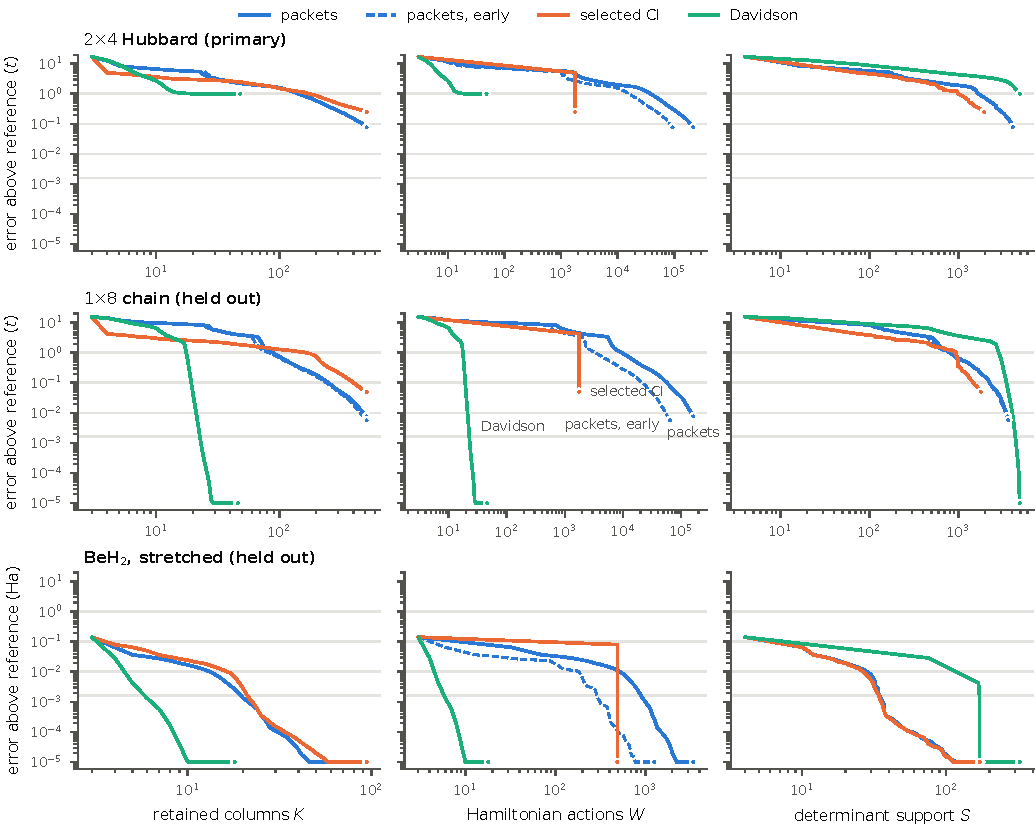
\includegraphics[width=\textwidth]{paper_assets/yardsticks.pdf}
\caption{A single set of trajectories, three yardsticks. Each curve is one arm's
error above the reference at every prefix, against retained columns (left),
cumulative Hamiltonian actions (middle) and determinant support (right), on
the primary lattice and both held-out inputs. Gray lines mark the declared
thresholds; dots mark each arm's last prefix; errors at rounding level are
drawn at the lower edge. Selected CI's vertical segment in the middle column is
its frame action table, paid at the first step. On the primary lattice
Davidson stops on an excited singlet.}
\label{fig:yardsticks}
\end{figure*}

\begin{table*}[t]
\caption{Columns $K$ and Hamiltonian actions $W$ at the first prefix within
each error threshold, and the error at the last prefix; units as in
Table~\ref{tab:inputs}. A dash marks a threshold not reached within the
budget. Final errors at or below the declared complete-span tolerance are
shown as such.}
\label{tab:thresholds}
\begin{ruledtabular}
\tightcolumns
\begin{tabular}{lrrrrrrrrr}
% source-git-blob-sha: 70da4d0015b3a81b50b63ea41cb8ce9c4799f6a8
% generator-git-blob-sha: 66427b7e92b19257102feee4147f2f3c2c4c0758
 & \multicolumn{2}{c}{$\le1$} & \multicolumn{2}{c}{$\le0.1$} & \multicolumn{2}{c}{$\le0.01$} & \multicolumn{2}{c}{$\le0.0016$} & \\
Arm & $K$ & $W$ & $K$ & $W$ & $K$ & $W$ & $K$ & $W$ & Final error \\
\hline
\multicolumn{10}{l}{\textit{$2{\times}4$ Hubbard}, primary; budget \ensuremath{512}, energies in $t$} \\
Packets & \ensuremath{145} & \ensuremath{38{,}345} & \ensuremath{473} & \ensuremath{194{,}347} & --- & --- & --- & --- & \ensuremath{0.0763} \\
Packets, early & \ensuremath{146} & \ensuremath{15{,}809} & \ensuremath{473} & \ensuremath{84{,}601} & --- & --- & --- & --- & \ensuremath{0.0766} \\
Selected CI & \ensuremath{174} & \ensuremath{1{,}764} & --- & --- & --- & --- & --- & --- & \ensuremath{0.248} \\
Davidson & \ensuremath{21} & \ensuremath{21} & --- & --- & --- & --- & --- & --- & \ensuremath{0.995} \\
\hline
\multicolumn{10}{l}{\textit{$1{\times}8$ Hubbard chain}, held-out lattice; budget \ensuremath{512}, energies in $t$} \\
Packets & \ensuremath{89} & \ensuremath{9{,}623} & \ensuremath{251} & \ensuremath{57{,}451} & \ensuremath{484} & \ensuremath{149{,}497} & --- & --- & \ensuremath{0.00762} \\
Packets, early & \ensuremath{83} & \ensuremath{3{,}459} & \ensuremath{242} & \ensuremath{21{,}658} & \ensuremath{454} & \ensuremath{54{,}394} & --- & --- & \ensuremath{0.00565} \\
Selected CI & \ensuremath{166} & \ensuremath{1{,}764} & \ensuremath{404} & \ensuremath{1{,}764} & --- & --- & --- & --- & \ensuremath{0.0496} \\
Davidson & \ensuremath{18} & \ensuremath{18} & \ensuremath{20} & \ensuremath{20} & \ensuremath{22} & \ensuremath{22} & \ensuremath{23} & \ensuremath{23} & \ensuremath{<10^{-8}} \\
\hline
\multicolumn{10}{l}{\textit{BeH$_2$, stretched}, held-out molecule; budget \ensuremath{490}, energies in Ha} \\
Packets & \ensuremath{3} & \ensuremath{3} & \ensuremath{4} & \ensuremath{32} & \ensuremath{14} & \ensuremath{575} & \ensuremath{20} & \ensuremath{928} & \ensuremath{<10^{-8}} \\
Packets, early & \ensuremath{3} & \ensuremath{3} & \ensuremath{4} & \ensuremath{6} & \ensuremath{14} & \ensuremath{190} & \ensuremath{20} & \ensuremath{297} & \ensuremath{<10^{-8}} \\
Selected CI & \ensuremath{3} & \ensuremath{3} & \ensuremath{4} & \ensuremath{490} & \ensuremath{17} & \ensuremath{490} & \ensuremath{22} & \ensuremath{490} & \ensuremath{<10^{-8}} \\
Davidson & \ensuremath{3} & \ensuremath{3} & \ensuremath{4} & \ensuremath{4} & \ensuremath{5} & \ensuremath{5} & \ensuremath{6} & \ensuremath{6} & \ensuremath{<10^{-8}} \\
\hline
\multicolumn{10}{l}{\textit{$2{\times}3$ Hubbard}, complete-span control; budget \ensuremath{175}, energies in $t$} \\
Packets & \ensuremath{21} & \ensuremath{669} & \ensuremath{55} & \ensuremath{2{,}715} & \ensuremath{78} & \ensuremath{4{,}178} & \ensuremath{102} & \ensuremath{5{,}544} & \ensuremath{<10^{-8}} \\
Packets, early & \ensuremath{21} & \ensuremath{266} & \ensuremath{55} & \ensuremath{1{,}256} & \ensuremath{80} & \ensuremath{1{,}843} & \ensuremath{105} & \ensuremath{2{,}469} & \ensuremath{<10^{-8}} \\
Selected CI & \ensuremath{16} & \ensuremath{175} & \ensuremath{61} & \ensuremath{175} & \ensuremath{103} & \ensuremath{175} & \ensuremath{135} & \ensuremath{175} & \ensuremath{<10^{-8}} \\
Davidson & \ensuremath{10} & \ensuremath{10} & \ensuremath{12} & \ensuremath{12} & \ensuremath{14} & \ensuremath{14} & \ensuremath{15} & \ensuremath{15} & \ensuremath{<10^{-8}} \\
\hline
\multicolumn{10}{l}{\textit{H$_2$O CAS(8e,6o)}, development control; budget \ensuremath{105}, energies in Ha} \\
Packets & \ensuremath{3} & \ensuremath{3} & \ensuremath{3} & \ensuremath{3} & \ensuremath{9} & \ensuremath{143} & \ensuremath{12} & \ensuremath{213} & \ensuremath{<10^{-8}} \\
Packets, early & \ensuremath{3} & \ensuremath{3} & \ensuremath{3} & \ensuremath{3} & \ensuremath{9} & \ensuremath{53} & \ensuremath{12} & \ensuremath{66} & \ensuremath{<10^{-8}} \\
Selected CI & \ensuremath{3} & \ensuremath{3} & \ensuremath{3} & \ensuremath{3} & \ensuremath{9} & \ensuremath{105} & \ensuremath{14} & \ensuremath{105} & \ensuremath{<10^{-8}} \\
Davidson & \ensuremath{3} & \ensuremath{3} & \ensuremath{3} & \ensuremath{3} & \ensuremath{4} & \ensuremath{4} & \ensuremath{5} & \ensuremath{5} & \ensuremath{<10^{-8}} \\

\end{tabular}
\end{ruledtabular}
\end{table*}

\subsection{Columns}
\label{sec:columns}

Table~\ref{tab:thresholds} gives every arm's columns and actions at each
threshold, and Table~\ref{tab:readouts} the declared readouts. On the primary
lattice, packets reach \pkThresholdOne\,$t$ in \pkPrimaryPacketsColumnsOne{} columns against
selected CI's \pkPrimarySciColumnsOne{}, a ratio of \pkPrimaryColumnRatioOne{},
above the declared \pkCompactRatio{}. Only packets reach \pkThresholdTenth\,$t$, after
\pkPrimaryPacketsColumnsTenth{} columns, and they end the budget
\pkPrimaryPacketsFinalError{}\,$t$ above the reference against selected CI's
\pkPrimarySciFinalError{}\,$t$. Packets thus win every frontier and miss the
ratio at the loosest threshold, while selected CI wins neither, so the
readout is mixed. On stretched BeH$_2$, packets reach \pkTightTarget{} in
\pkBerylliumPacketsColumnsTight{} columns against selected CI's
\pkBerylliumSciColumnsTight{}, a ratio of \pkBerylliumColumnRatioTight{}:
mixed again. Only on the held-out chain do packets meet the rule, needing
\pkChainPacketsColumns{} columns to reach \pkChainPacketThresholds\,$t$
against selected CI's \pkChainSciColumns{}, with the last threshold out of
selected CI's reach.
The decisive inputs therefore read mixed, packets, mixed, and the declared
answer is that packets add no column compactness.

\begin{table*}[t]
\caption{Declared readouts. Columns: which arm is more column-compact, packets
against selected CI. Work: the action penalty of the more compact arm. Early:
the early policy against the declared band. Davidson: whether it reaches every
threshold in fewer columns than both restricted arms. Roles are as in
Table~\ref{tab:inputs}.}
\label{tab:readouts}
\begin{ruledtabular}
\tightcolumns
\begin{tabular}{lllll}
Input & Columns & Work & Early & Davidson \\
\hline
% source-git-blob-sha: 70da4d0015b3a81b50b63ea41cb8ce9c4799f6a8
% generator-git-blob-sha: 66427b7e92b19257102feee4147f2f3c2c4c0758
$2{\times}4$ Hubbard & mixed & --- & within band & excited root \\
$1{\times}8$ Hubbard chain & packets & packets $\ge$\ensuremath{5.4}$\times$ actions & outside band, lower error & fewer at every threshold \\
BeH$_2$, stretched & mixed & --- & within band & ties at the start span \\
$2{\times}3$ Hubbard & mixed & --- & outside band & fewer at every threshold \\
H$_2$O CAS(8e,6o) & mixed & --- & within band & ties at the start span \\

\end{tabular}
\end{ruledtabular}
\end{table*}

The early policy tracks the exhaustive one within the declared band on the
primary lattice and on BeH$_2$. On the chain it falls outside the band in the
favourable direction, ending \pkChainEarlyFinalError{}\,$t$ above the
reference against exhaustive's \pkChainPacketsFinalError{}\,$t$; on the
\pkLadderName{} control the frontier differences change sign.

Davidson, wherever it reaches the ground state, needs no more columns than
either restricted arm at any threshold, and far fewer at tight ones. On the
chain it reaches \pkThresholdTight\,$t$ in
\pkChainDavidsonColumnsTight{} columns, a threshold neither restricted arm
reaches within its budget; on BeH$_2$ it reaches \pkTightTarget{} in
\pkBerylliumDavidsonColumnsTight{} columns, and on the \pkLadderName{} in
\pkLadderDavidsonColumnsTight{} against \pkLadderPacketsColumnsTight{} for
packets and \pkLadderSciColumnsTight{} for selected CI. Every arm reaches the
reference on both complete-span controls. The packets-versus-selected-CI
question is therefore a question about bounded-support compactness only: when
column support is free, the unrestricted direction is far more compact than
either.

\subsection{Actions}
\label{sec:actions}

Counting Hamiltonian actions turns the bounded-support ranking around. Where
packets win on columns, on the chain, they need \pkChainMinActionRatio{} or
more times selected CI's actions at every threshold both reach. On the
primary lattice they end the budget with \pkPrimaryPacketsActions{} actions
against selected CI's \pkPrimarySciActions{}, about \pkPrimaryActionRatio{}
times as many; the early policy reaches the same columns with
\pkPrimaryEarlyActions{}, a factor of \pkPrimaryEarlyActionFactor{} fewer. The
single exception is an early BeH$_2$ threshold: packets reach \pkThresholdTenth\,Ha after
\pkBerylliumColumnsTenth{} columns and \pkBerylliumPacketsActionsTenth{}
actions, before selected CI's \pkBerylliumSciActionsTenth{}-action table has
paid for itself.

The count hides an asymmetry. Selected CI's \pkPrimarySciActions{} actions are
its whole frame action table, computed once and stored; on every decisive
input its final count equals the singlet-frame dimension. Packets instead
apply $H$ to a new direction for every group at every step, because each
direction depends on the current residual. The cheapest yardstick for selected
CI here is therefore a memory cost in disguise, a dense table of $F_s$ sector
vectors, which does not survive growth of the sector. Davidson spends one
action per column and leads on actions wherever it reaches a threshold.

\subsection{Support}
\label{sec:support}

\begin{table}[t]
\caption{Determinant support $S$ at the first prefix within each threshold
(units as in Table~\ref{tab:inputs}), and at Davidson's last prefix, where all
arms are compared at the same number of columns.}
\label{tab:support}
\begin{ruledtabular}
\tightcolumns
\begin{tabular}{lrrrrr}
% source-git-blob-sha: 70da4d0015b3a81b50b63ea41cb8ce9c4799f6a8
% generator-git-blob-sha: daabb897d72e67a564233dae3804d4d1e6607db2
Arm & $\le1$ & $\le0.1$ & $\le0.01$ & $\le0.0016$ & Matched $K$ \\
\hline
\multicolumn{6}{l}{\textit{$2{\times}4$ Hubbard}; matched at $K=\ensuremath{48}$} \\
Packets & \ensuremath{1{,}696} & \ensuremath{4{,}000} & --- & --- & \ensuremath{676} \\
Packets, early & \ensuremath{1{,}700} & \ensuremath{3{,}986} & --- & --- & \ensuremath{654} \\
Selected CI & \ensuremath{1{,}010} & --- & --- & --- & \ensuremath{396} \\
Davidson & \ensuremath{4{,}720} & --- & --- & --- & \ensuremath{4{,}900} \\
\hline
\multicolumn{6}{l}{\textit{$1{\times}8$ Hubbard chain}; matched at $K=\ensuremath{46}$} \\
Packets & \ensuremath{842} & \ensuremath{2{,}244} & \ensuremath{3{,}496} & --- & \ensuremath{308} \\
Packets, early & \ensuremath{794} & \ensuremath{2{,}236} & \ensuremath{3{,}414} & --- & \ensuremath{296} \\
Selected CI & \ensuremath{942} & \ensuremath{1{,}474} & --- & --- & \ensuremath{482} \\
Davidson & \ensuremath{3{,}023} & \ensuremath{3{,}710} & \ensuremath{4{,}239} & \ensuremath{4{,}436} & \ensuremath{4{,}900} \\
\hline
\multicolumn{6}{l}{\textit{BeH$_2$, stretched}; matched at $K=\ensuremath{18}$} \\
Packets & \ensuremath{4} & \ensuremath{10} & \ensuremath{30} & \ensuremath{35} & \ensuremath{34} \\
Packets, early & \ensuremath{4} & \ensuremath{10} & \ensuremath{30} & \ensuremath{35} & \ensuremath{34} \\
Selected CI & \ensuremath{4} & \ensuremath{8} & \ensuremath{27} & \ensuremath{35} & \ensuremath{29} \\
Davidson & \ensuremath{4} & \ensuremath{75} & \ensuremath{168} & \ensuremath{171} & \ensuremath{325} \\

\end{tabular}
\end{ruledtabular}
\end{table}

Table~\ref{tab:support} gives the support of each span. At \pkThresholdOne\,$t$ on the
primary lattice, packets span \pkPrimaryPacketsSupportOne{} determinants and
selected CI \pkPrimarySciSupportOne{}; Davidson reaches the same threshold with
\pkPrimaryDavidsonColumnsOne{} columns spread over
\pkPrimaryDavidsonSupportOne{} of the \pkPrimaryDeterminants{} determinants.
Compared at Davidson's final \pkPrimaryMatchedColumns{} columns, packets span
\pkPrimaryPacketsSupportMatched{} determinants, selected CI
\pkPrimarySciSupportMatched{}, and Davidson the entire sector. On the chain,
packets lead on support at \pkThresholdOne\,$t$, with \pkChainPacketsSupportOne{}
determinants against \pkChainSciSupportOne{}, and selected CI leads at
\pkThresholdTenth\,$t$, with \pkChainSciSupportTenth{} against
\pkChainPacketsSupportTenth{}, while Davidson reaches \pkThresholdTight\,$t$
with \pkChainDavidsonColumnsTight{} columns spread over
\pkChainDavidsonSupportTight{} determinants. On BeH$_2$ the two meet at \pkTightTarget{} on
\pkBerylliumPacketsSupportTight{} determinants each, while Davidson needs
\pkBerylliumDavidsonSupportTight{}.

Support counts carry one caveat. Packet and Davidson directions on the
molecular inputs, and Davidson's directions on the primary lattice, hold
amplitudes near the \pkSupportTolerance{} counting threshold, because
normalizing a small projected direction amplifies rounding. Their recorded
counts reproduce exactly, but an independent computation of the same span can
count a few percent differently; the checker brackets each recorded count
between the independent counts at neighbouring thresholds. Selected-CI columns
are exact CSFs, and the packet spans on the lattices hold no amplitudes in that
band, so their recorded and independent counts agree exactly.

\subsection{Who leads depends on the yardstick}

\begin{table*}[t]
\caption{Leaders by yardstick among the three growth rules (P: packets, S:
selected CI, D: Davidson) at every threshold some rule reaches beyond the
starting span, with the leading value in parentheses; ties list every leader.
The last three columns compare packets with selected CI where both reach the
threshold.}
\label{tab:leaders}
\begin{ruledtabular}
\begin{tabular}{llllllll}
% source-git-blob-sha: 70da4d0015b3a81b50b63ea41cb8ce9c4799f6a8
% generator-git-blob-sha: 66427b7e92b19257102feee4147f2f3c2c4c0758
Input & $\le$ & Columns & Actions & Support & $K_P/K_S$ & $W_P/W_S$ & $S_P/S_S$ \\
\hline
$2{\times}4$ Hubbard & \ensuremath{1} & D (\ensuremath{21}) & D (\ensuremath{21}) & S (\ensuremath{1{,}010}) & \ensuremath{0.83} & \ensuremath{21.74} & \ensuremath{1.68} \\
$2{\times}4$ Hubbard & \ensuremath{0.1} & P (\ensuremath{473}) & P (\ensuremath{194{,}347}) & P (\ensuremath{4{,}000}) & --- & --- & --- \\
$1{\times}8$ Hubbard chain & \ensuremath{1} & D (\ensuremath{18}) & D (\ensuremath{18}) & P (\ensuremath{842}) & \ensuremath{0.54} & \ensuremath{5.46} & \ensuremath{0.89} \\
$1{\times}8$ Hubbard chain & \ensuremath{0.1} & D (\ensuremath{20}) & D (\ensuremath{20}) & S (\ensuremath{1{,}474}) & \ensuremath{0.62} & \ensuremath{32.57} & \ensuremath{1.52} \\
$1{\times}8$ Hubbard chain & \ensuremath{0.01} & D (\ensuremath{22}) & D (\ensuremath{22}) & P (\ensuremath{3{,}496}) & --- & --- & --- \\
$1{\times}8$ Hubbard chain & \ensuremath{0.0016} & D (\ensuremath{23}) & D (\ensuremath{23}) & D (\ensuremath{4{,}436}) & --- & --- & --- \\
BeH$_2$, stretched & \ensuremath{0.1} & P (\ensuremath{4}), S (\ensuremath{4}), D (\ensuremath{4}) & D (\ensuremath{4}) & S (\ensuremath{8}) & \ensuremath{1.00} & \ensuremath{0.07} & \ensuremath{1.25} \\
BeH$_2$, stretched & \ensuremath{0.01} & D (\ensuremath{5}) & D (\ensuremath{5}) & S (\ensuremath{27}) & \ensuremath{0.82} & \ensuremath{1.17} & \ensuremath{1.11} \\
BeH$_2$, stretched & \ensuremath{0.0016} & D (\ensuremath{6}) & D (\ensuremath{6}) & P (\ensuremath{35}), S (\ensuremath{35}) & \ensuremath{0.91} & \ensuremath{1.89} & \ensuremath{1.00} \\

\end{tabular}
\end{ruledtabular}
\end{table*}


Table~\ref{tab:leaders} and Fig.~\ref{fig:yardsticks} collect the pattern.
Wherever Davidson reaches a threshold that another rule also reaches, it leads
in columns and in actions, and it never leads in support. Between the two
bounded-support rules, packets need no more columns than selected CI at any
shared threshold, but clear the declared margin only on the chain; selected CI
leads in actions at every shared threshold but the early BeH$_2$ one; and the
support lead changes hands from threshold to threshold. No rule leads on all three yardsticks at any shared threshold, so
a ranking by one of them says little about the others. That is the paper's
central observation, and it is why the declared rule had to name its yardstick
before the trajectories existed.

\subsection{The Davidson reference on the primary lattice}
\label{sec:davidson}

On the primary lattice, Davidson stopped after \pkPrimaryDavidsonStopColumns{}
columns because no admissible direction remained: the projected
preconditioned residual fell below the direction cutoff while the residual
norm stood at \pkPrimaryDavidsonResidual{}, on a Ritz state
\pkPrimaryDavidsonError{}\,$t$ above the reference with ground-space overlap
\pkPrimaryDavidsonOverlap{}. That is a numerically converged excited singlet,
and not the first one: the gap from the ground singlet to
the next singlet is only \pkPrimaryGap{}\,$t$. The shared starting span
carries a ground-state weight of \pkPrimaryStartWeight{} on this input. On the
chain the weight is at rounding level (\pkChainStartWeight{}), yet Davidson
reaches the ground state there, presumably because rounding seeds the missing
component and the iteration amplifies it. The starting weight alone therefore
does not predict the outcome.

The declaration named only residual-tolerance stops as confinement, so the
verdict follows the declared fallback: on the primary lattice Davidson does not
reach every threshold. The episode illustrates a familiar limit with a fresh
example. A small residual guarantees that an eigenvalue lies nearby, not that
it is the lowest one~\cite{weinstein1934modified}; fewer columns to a
converged eigenpair is not the same as fewer columns to the ground state. A
later bounded sector solver in the toolkit keeps this archived vector as a
regression case, recovers the ground singlet from independent starts, and
reports a state like this one as numerically converged with its root
unresolved. That solver was not part of the comparison.

\section{Making the losing arm cheaper}
\label{sec:ledger}

Before and after the column comparison, separately declared campaigns
reduced the cost of the packet arm (Table~\ref{tab:ledger}). Each declared in
advance what equivalence it required and what improvement would justify a
change of default, and each was run under the same fresh-process discipline.

\begin{table*}[t]
\caption{Engineering on the packet arm, each change in its own declared
campaign on the primary lattice at a budget of \pkLargeBudget{} columns,
under the exhaustive policy except for the shortlist, which is itself a
screening policy. Times are medians of setup plus solver in
seconds, and peak resident memory is in MiB; both compare within one
campaign only, because harness changes moved the baselines between campaigns.
The outcome is the campaign's declared promotion verdict.
$^{a}$Masked by a floor from the provenance preflight; solver-only memory was
not measured.}
\label{tab:ledger}
\begin{ruledtabular}
\begin{tabular}{llllll}
Change & Trajectory & Work & Time (s) & Memory (MiB) & Outcome \\
\hline
% source-git-blob-sha: 6e2f6da87ed8f0a0ebfd9af688a3a2574020b6e0
% source-git-blob-sha: 178bd5fd9c391703a17241da8c3f9196a42cc3a0
% source-git-blob-sha: 3a9a7d874cb53619293f51cf0a6a51809234587d
% source-git-blob-sha: 55418ea5bd2206a7e012b32493c804c66f1633bb
% generator-git-blob-sha: 66427b7e92b19257102feee4147f2f3c2c4c0758
Frame action reuse & identical selections & \ensuremath{10{,}841}$\to$\ensuremath{1{,}301} actions & \ensuremath{27.9}$\to$\ensuremath{43.4} & \ensuremath{684}$\to$\ensuremath{897} & kept experimental \\
Residual shortlist & heuristic; trajectory changes & \ensuremath{10{,}838}$\to$\ensuremath{4{,}466} scores & \ensuremath{27.9}$\to$\ensuremath{26.2} & \ensuremath{684}$\to$\ensuremath{684} & kept experimental \\
Sparse setup & identical up to phase & --- & \ensuremath{27.4}$\to$\ensuremath{25.8} & \ensuremath{686}$\to$\ensuremath{181}$^{a}$ & speed clause fails \\
Projection caches & bitwise identical & --- & \ensuremath{24.8}$\to$\ensuremath{13.8} & \ensuremath{138}$\to$\ensuremath{144} & memory clause fails \\
Frame coordinates & shortlist order differs & --- & \ensuremath{29.1}$\to$\ensuremath{14.5} & \ensuremath{97}$\to$\ensuremath{97} & equivalence fails \\

\end{tabular}
\end{ruledtabular}
\end{table*}

\emph{Fixed-frame action reuse} keeps the action of every frame column it
touches and forms each packet direction's action by linearity. It preserves
the selections exactly. On water it cut the actions to the
\pkTightTarget{} target from \pkWaterPacketActions{} to
\pkWaterReuseActions{}; on the primary lattice it cut them from
\pkReuseActionsBefore{} to \pkReuseActionsAfter{}, while the time rose from
\pkReuseSecondsBefore{} to \pkReuseSecondsAfter{}\,s and peak memory from
\pkReuseRssBefore{} to \pkReuseRssAfter{}\,MiB. The cache approaches the
complete frame action table, so reuse turns the packets' actions into the
same stored table that selected CI keeps---and selected CI finished the same
budget in \pkLargeSciSeconds{}\,s.

\emph{Residual shortlisting} scores only the groups holding most of the
residual mass and audits the rest periodically. It cut exact scores on water
from \pkWaterPacketScores{} to \pkWaterShortlistScores{}, but it is a heuristic
that changes the trajectory: on the primary lattice it ended
\pkShortlistErrorChange{} higher, and in its later early-marking form, on the
held-out \pkLadderName{}, it missed the winner in \pkLadderEarlyMissed{} of \pkLadderEarlyAudits{} audits and ended
\pkLadderEarlyErrorChange{} higher.

\emph{Sparse setup} assembles the sector Hamiltonian directly in sparse form
and builds spin blocks locally, removing the dense full-sector setup. Peak
memory fell from \pkSparseRssBefore{} to \pkSparseRssAfter{}\,MiB, a value
masked by the provenance floor, but the time fell by only
\pkSparseReduction{} against the declared \pkSparseDeclaredReduction{}, so the
speed clause failed.

\emph{Exact projection caches} keep one adjoint of the accepted span per step
and fixed copies of the group blocks per run. All \pkCacheCells{} cells
produced only \pkCachePayloads{} distinct trajectories, bitwise identical
across cache modes within each input and policy. On the primary lattice the
combined caches cut time by \pkCacheReduction{}, beyond the declared
\pkCacheMinimumReduction{}, but raised peak memory by \pkCacheRssGrowth{}
against a declared ceiling of no increase. The joint clause failed and the
caches stayed opt-in.

\emph{Frame-coordinate projection} projects in the coordinates of the fixed
frame, using $(I-VV^\dagger)Fa=F(I-CC^\dagger)a$ with $C=F^\dagger V$, which is
exact in arithmetic. It cut time by \pkCoordinateExhaustiveReduction{} under
the exhaustive policy and \pkCoordinateEarlyReduction{} under the early one,
with memory flat. But it changes the order of floating-point reductions, and
under the early policy two near-tied groups swapped places in the ordered
shortlist at steps \pkCoordinateSwapSteps{}, in every repetition, although
the shortlist members and every selected candidate agreed. The declared
criterion was exact ordered-shortlist equality, so the comparison failed.

Two lessons follow. First, none of these changes moves $K$, and $K$ was the
declared question. The column comparison ran with the exact caches enabled,
so its packet columns are exactly the uncached ones. Its packet action counts
include no action reuse; reuse would have cut them by storing a frame action
table, which is what selected CI already does. Speeding up an arm does not
change which arm needs fewer columns. Second,
``exact'' needs a declared meaning. Bitwise payload identity, identical
selections, identical ordered shortlists, and identical physical rays up to a
global phase are different criteria. Frame-coordinate projection is exact in
arithmetic and fails the strictest of them; naming the criterion before
measuring the speed-up is what kept a halved run time from being promoted on a
criterion relaxed after the fact. Once the column comparison was in, the
project closed the residual-packet line. The frame-coordinate comparison,
already declared, was completed and recorded; further speed-up work and the
promotion of the opt-in caches were dropped, and the shipped solver and its
defaults were left unchanged.

\section{Discussion}
\label{sec:discussion}

\subsection{Compactness needs a declared cost model}

A statement that one subspace is more compact than another is a statement
about a cost model, whether or not the model is written down. Suppose the cost
of a run is some increasing function $C(K,W,S)$. If $C$ depends on columns
alone, Davidson wins wherever it finds the right root, and packets are not in
contention. If $C$ is dominated by actions, Davidson wins again, followed by
selected CI for as long as its action table fits in memory. Only if $C$
charges for column support does the comparison between the bounded-support
rules become the interesting one---and there the data show packets and
selected CI trading the lead.

Packets would pay off under a model with three properties at once: columns
are expensive, column support is expensive, and Hamiltonian actions during
selection are cheap relative to both. A measured setting in which every
column must be prepared and every pair of columns measured, while candidate
scoring stays classical, is the obvious candidate. These simulations cannot
test it: they count actions on explicit vectors and measure nothing. The
project's plan therefore sets the condition for reopening the line as a new
declaration whose cost model prices bounded column support, for example
through measured matrix elements.

\subsection{Relation to sampled-determinant methods}

In quantum-selected CI and sample-based quantum diagonalization, the basis
consists of determinants, so $K=S$ and the subspace dimension is also the
support~\cite{kanno2026qsci,robledomoreno2025sqd}. Those methods escape the
tension studied here by construction, and the price of their columns sits in
the sampling that finds them. Methods that dress or combine determinants into
richer columns, of which packets are one, re-open the gap between $K$ and $S$
and owe a statement of which one they are reducing.

\subsection{Roots and residuals}

The Davidson result on the primary lattice is a reminder that a residual-based
stop certifies an eigenpair, not the ground state. A column comparison that
ranks rules by the dimension at which they converge needs a root diagnostic
reported beside it; the declared overlap diagnostic is what made the excited
singlet visible here rather than a mysteriously flat error curve.

\section{Scope and limitations}
\label{sec:limitations}

The sectors are small, with at most \pkPrimaryDeterminants{} determinants, and
every column is an explicit sector vector. All arms share one starting
protocol, a \pkStartSpace{} singlet span with frozen outer orbitals, and one
preconditioner. The selected CI is greedy and spin-adapted, not CIPSI or
heat-bath CI with perturbative corrections~\cite{huron1973cipsi,
holmes2016hci}, and its action table would not fit on larger sectors. The
Davidson arm targets one root without restarts or root tracking. The held-out
inputs were held out from the design of this comparison but are known
Hamiltonians, not blind data. Thresholds are absolute and differ in meaning
between lattice and molecular units. Timings come from \pkMinRepeats{} or \pkMaxRepeats{}
repetitions on one host and are descriptive; resident memory is a process
high-water mark. Support counts on molecular inputs are sensitive to rounding
at the counting threshold. No quantum measurement, device, noise model or
asymptotic scaling is involved, and no hardware or quantum-advantage claim
follows from any result here.

\section{Reproducibility}
\label{sec:reproducibility}

Every number in the body and tables is generated from committed records by
the paper's table generator, which reads the declared comparison's
content-addressed trajectories and the records of the engineering campaigns
without recomputing any result. Where the prose states a pattern rather than a
number---which inputs read mixed, that Davidson stopped on an excited root,
that caches left trajectories bitwise identical, that no rule leads on all
three yardsticks---the generator asserts it against the record and refuses to
emit tables that would contradict the text. The start-span weights come from
the independent checker's own functions, stored with the identity of the
record they were computed from. A manuscript checker regenerates every
fragment and compares it byte for byte, rejects any numeral typed into the
prose, and checks the figure manifest against the digests of its inputs.

\section*{Code and data availability}

The toolkit source, the declarations, records, checkers and summaries of every
campaign quoted here, and the generators and checker of this manuscript are
versioned together in one Apache-licensed repository at
\url{https://github.com/gutama/clifford_qc}. The manuscript sources are under
\texttt{paper\_compactness/}, and \texttt{REPRODUCING.md} records the
environment each record was produced in. Rebuilding the paper requires no data
outside that repository.

\begin{acknowledgments}
We thank the developers of NumPy and SciPy~\cite{harris2020numpy,
virtanen2020scipy}, on which every calculation here runs.
\end{acknowledgments}

\bibliographystyle{apsrev4-2}
\bibliography{references}

\end{document}
